\documentclass[xcolor=pdftex,dvipsnames,table,mathserif,aspectratio=169]{beamer}
\usetheme{metropolis}
%\usetheme{Darmstadt}
%\usepackage{times}
%\usefonttheme{structurebold}

\usepackage[english]{babel}
%\usepackage[table]{xcolor}
\usepackage{pgf,pgfarrows,pgfnodes,pgfautomata,pgfheaps}
\usepackage{amsmath,amssymb,setspace,centernot}
\usepackage[latin1]{inputenc}
\usepackage[T1]{fontenc}
\usepackage{relsize}
\usepackage{pdfpages}
\usepackage[absolute,overlay]{textpos} 

\DeclareMathSizes{10}{10}{6}{6} 


\title [Dynamic Demand I]{Dynamic Demand I:\\
 Durable Goods }
\author{C.Conlon}
\institute{Grad IO}
\date{\today}
\setbeamerfont{equation}{size=\tiny}
\begin{document}

\begin{frame}
\titlepage
\end{frame}

\begin{frame}{Today's Readings}
\begin{itemize}
\item Melnikov (Yale PhD Thesis 2001)
\item Gowrisankaran Rysman (JPE)
\item Hendel and Nevo (Econometrica )
\end{itemize}
\end{frame}


\begin{frame}
\frametitle{G+R: Assumptions}
 We can formally write down a dynamic programming problem that consumers solve:
\begin{eqnarray*}
V_i(f_{i0t},\varepsilon_{i t}, \Omega_t) &=& \max \{ f_{i0t} + \beta E_{\Omega}[ E_{\varepsilon} V_i (f_{i0t}, \varepsilon_{it}, \Omega_{t+1}) |\Omega_{t} ] ,\\
&& \max_j f_{ijt}  -\alpha_i p_{jt} + \beta E_{\Omega}[ E_{\varepsilon} V_i (f_{ijt}, \varepsilon_{it}, \Omega_{t+1}) |\Omega_{t} ]  \}
\end{eqnarray*}
For a dynamic model to make sense we may want to place some restrictions:
\begin{itemize}
\item Rational Expectations
\item Dynamic Consistency
\item Law of motion for consumer types: $w_{i,t+1} =h(w_{i,t},s_{ijt})$ 
\end{itemize}
\end{frame}

\begin{frame}
\frametitle{Replacement Problem}
This Bellman has defined a \textit{Replacement Problem}.
\begin{itemize}
\item You own a single durable good with the option to \textit{upgrade} each period.
\item When you upgrade \alert{you throw away the old durable and get nothing in exchange}.
\item After a purchase $j$  you receive flow utility $f_{i0t+1} = f_{ijt}$ each period if you don't make a new purchase.
\item We could add in depreciation or probabilistic failure if we wanted to.
\item No resale market (reasonable for high-tech).
\end{itemize}
\end{frame}





\begin{frame}
\frametitle{Inclusive Value}
 Helpful to write: $EV_i(\Omega_t)= \int V_i(\varepsilon_{it},  \Omega_t)f(\varepsilon)$ \alert{Rust's Trick}
\begin{eqnarray*}
V_i(f_{i0t},\varepsilon_{i t}, \Omega_t) &=& \max \{ f_{i0t} + \beta E_{\Omega}[ EV_i (f_{i0t}, \Omega_{t+1}) |\Omega_{t} ] + \varepsilon_{i0t},\\
&& \max_j f_{ijt}  -\alpha_i p_{jt} + \beta E_{\Omega}[ E V_i (f_{ijt}, \Omega_{t+1}) |\Omega_{t}] + \varepsilon_{ijt}  \}
\end{eqnarray*}
We can write the \alert{ex-ante} expected utility of purchasing in period $t$ without having to condition on which good you purchase:
\begin{eqnarray*} 
\delta_{i}(\Omega_t) &=& E_{\varepsilon} [ \max_j f_{ijt}  -\alpha_i p_{jt} + \beta E_{\Omega}[ E V_i (f_{ijt}, \Omega_{t+1}) |\Omega_{t}] + \varepsilon_{ijt}]  \\
&=& \log \left( \sum_j \exp[ f_{ijt}  -\alpha_i p_{jt} + \beta E_{\Omega}[ E V_i (f_{ijt}, \Omega_{t+1}) |\Omega_{t}] ]  \right)
\end{eqnarray*}
\end{frame}

\begin{frame}
\frametitle{Inclusive Value Sufficiency}
\begin{eqnarray*}
\small EV_i(f_{i0}, \Omega) = \log\left( \exp[ f_{i0} + \beta E_{\Omega'}[ EV_i (f_{i0}, \Omega') |\Omega]] + \exp(\delta_i(\Omega))  \right) + \eta
\end{eqnarray*}
\footnotesize 
\alert{where $\eta = 0.577215665$ (Euler's Constant).}\\
\normalsize
The fact that the expected value function depends recursively on itself and $\delta_{i}(\Omega_t)$ (Inclusive Value) leads to the following assumption.
\begin{block}{Inclusive Value Sufficiency}
If $\delta_i(\Omega) = \delta_i(\tilde{\Omega})$ then $g(\delta_i(\Omega') | \Omega)= g(\delta_i(\tilde{\Omega'}) | \tilde{\Omega})$ for all $\Omega,\tilde{\Omega}$.
\end{block}
\begin{itemize}
\item The idea is that $\delta$ tells me everything about the future evolution of the states
\item More restrictive than it looks.  $\delta$ is low because quality is low? or because prices are high? Is this the result of a dynamic pricing equilibrium? (No!)
\end{itemize}
\end{frame}

\begin{frame}
\frametitle{Inclusive Value Sufficiency}
Under IVS the problem reduces to
\begin{eqnarray*}
EV_i(f_{i0}, \alert{\delta_i}) &=& \log\left[ \exp( f_{i0} + \beta E_{\Omega'}[ EV_i (f_{i0}, \alert{\delta_i'}) |\alert{\delta_i}] )+ \exp(\alert{\delta_i})  \right]\\
\alert{\delta_{i}} &=& \log \left( \sum_j \exp[ f_{ijt}  -\alpha_i p_{jt} + \beta E_{\alert{\delta'}}[ E V_i (f_{ijt}, \alert{\delta_i'}) |\alert{\delta_i} ]  \right)
\end{eqnarray*}
The idea is that the inclusive value $\delta_{it}$ IS the state space, along with his current holding of the durable $f_{i0t}$.
\end{frame}


\begin{frame}
\frametitle{Rational Expectations}
We still have the expectation to deal with: 
\begin{eqnarray*}
E_{\alert{\delta'}}[ E V_i (f_{ijt}, \alert{\delta_i'}) |\alert{\delta_i} ]
\end{eqnarray*}
We need to take a stand on $g_i(\delta_i' | \delta_i)$ the anticipated law of motion for $\delta_i$.  G\&R assume it follows an $AR(1)$ process.
\begin{eqnarray*}
\delta_{it+1} = \gamma_0 + \gamma_1 \delta_{it} + \nu_{it} \mbox{ with } \nu_{it} \sim N(0,\sigma_{\nu}^2)
\end{eqnarray*}
If we see $\delta_{it}$ we could just run the $AR(1)$ regression to get consumer belief's $\hat{\gamma}$
\end{frame}


\begin{frame}
\frametitle{Rational Expectations-Interpolation}
I still haven't told you how to compute
\begin{eqnarray*}
E_{\delta'}[ E V_i (f_{ijt}, \delta_i') |\delta_i ,\gamma]= \int EV_i(f_{ijt},\delta_{i}') g(\delta' | \delta,\gamma)
\end{eqnarray*}
\vspace{-0.5cm}
\begin{enumerate}
\item We need to integrate $EV(f_{ijt},\delta_i)$ (a function) over a normal density.
\item But we don't observe $EV(f_{ijt},\delta_i)$ everywhere, only on the grid points of our state space.
\item We can fit a linear function, cubic spline, etc. over $\delta_i$ to $EV_i$ at each value of $f_{ijt}$ on our grid.
\item  We need to \alert{interpolate} $\widehat{EV}_i(\delta_i^s)$ (Linear, Cubic Spline, etc.)
\item We might as well interpolate the function at the \textit{Gauss-Hermite} quadrature nodes and weights, recentered at $\gamma_0 + \gamma_1 \delta$ in order to reduce the number of places we interpolate $\widehat{EV_i}$.
\end{enumerate}
\end{frame}

\begin{frame}
\frametitle{Rational Expectations-Alternative}
There is an alternative method that is likely to be less accurate
\begin{eqnarray*}
E_{\delta'}[ E V_i (f_{ijt}, \delta_i') |\delta_i, \gamma ]= \int EV_i(f_{ijt},\delta_{i}') g(\delta' | \delta, \gamma)
\end{eqnarray*}
\begin{enumerate}
\item We need to integrate $EV(f_{ijt},\delta_i)$ (a function) over a normal density but we only see it at the grid points of our state space.
\item We could \alert{discretize $g(\delta' | \delta,\gamma)$} so that it is a valid markov transition probability matrix (TPM) evaluated only at the grid points.
\item Now computing the expectation is just matrix multiplication.
\end{enumerate}
I am a bit nervous about whether two discrete approximations will get the continuous integral correct.
\end{frame}

\begin{frame}{The Estimation Problem}
We need to solve $\forall i, t $:
\begin{eqnarray*}
S_{jt} &=& \sum_i w_i s_{ijt}(f_{i0t},\delta_{it})\\
f_{ijt} &=& \overline{\alpha} x_{jt} + \xi_{jt} + \sum_l \sigma_l x_{jl} \nu_{il} \\
s_{ijt}(f_{i0t},\delta_{it}) &=& \frac{\exp[f_{ijt} - \alpha_i p_{jt} + \beta E_{\Omega'}[ EV_i (f_{ijt}, \delta_i') |\delta_i] }{\exp [EV_i(f_{i0t},\delta_{it}) ]}\\
EV_i(f_{i0}, \delta_i) &=& \log\left[ \exp( f_{i0} + \beta E_{\Omega'}[ EV_i (f_{i0}, \delta_i') |\delta_i] )+ \exp(\delta_i)  \right]\\
\delta_{i}(EV_i) &=& \log \left( \sum_j \exp[ f_{ijt}  -\alpha_i p_{jt} + \beta E_{\delta'}[ E V_i (f_{ijt}, \delta_i') |\delta_i ]  \right)\\
E[\delta_{it+1} | \delta_{it}] &=& \gamma_0 + \gamma_1 \delta_{it}\\
w_{i,t+1} &=&h(w_{i,t},s_{ijt})\\
\end{eqnarray*}
\end{frame}

\begin{frame}{The Estimation Problem}
\begin{enumerate}
\item Like BLP we guess the nonlinear parameters of the model $\theta$
\item For a guess of the $\xi_{jt}$'s we can solve for $EV_i$ by iteratively computing $\delta$, and running the $\gamma$ regression for each $i$ and spline/interpolating to compute $E[EV_i]$. (Inner Loop)
\item G\&R show how the contraction mapping of BLP can be modified to find a fixed point of the $\delta,\xi,\gamma$ relationship to find $f_{ijt}$ (Middle Loop).
\item We need to make sure to update the $w_{i,t}$ via $h(\cdot)$.  (This is a TPM that tells maps the transition probabilities of type $i$ holding $f_{i0t}$ to $f_{i0,t+1}$).
\item Once we've solved this whole system of equations, we use $\xi$ to form moments just like BLP and do GMM. (Outer Loop)
\end{enumerate}
\end{frame}

\begin{frame}{G\&R Parameters}
\begin{figure}[htbp]
\begin{center}
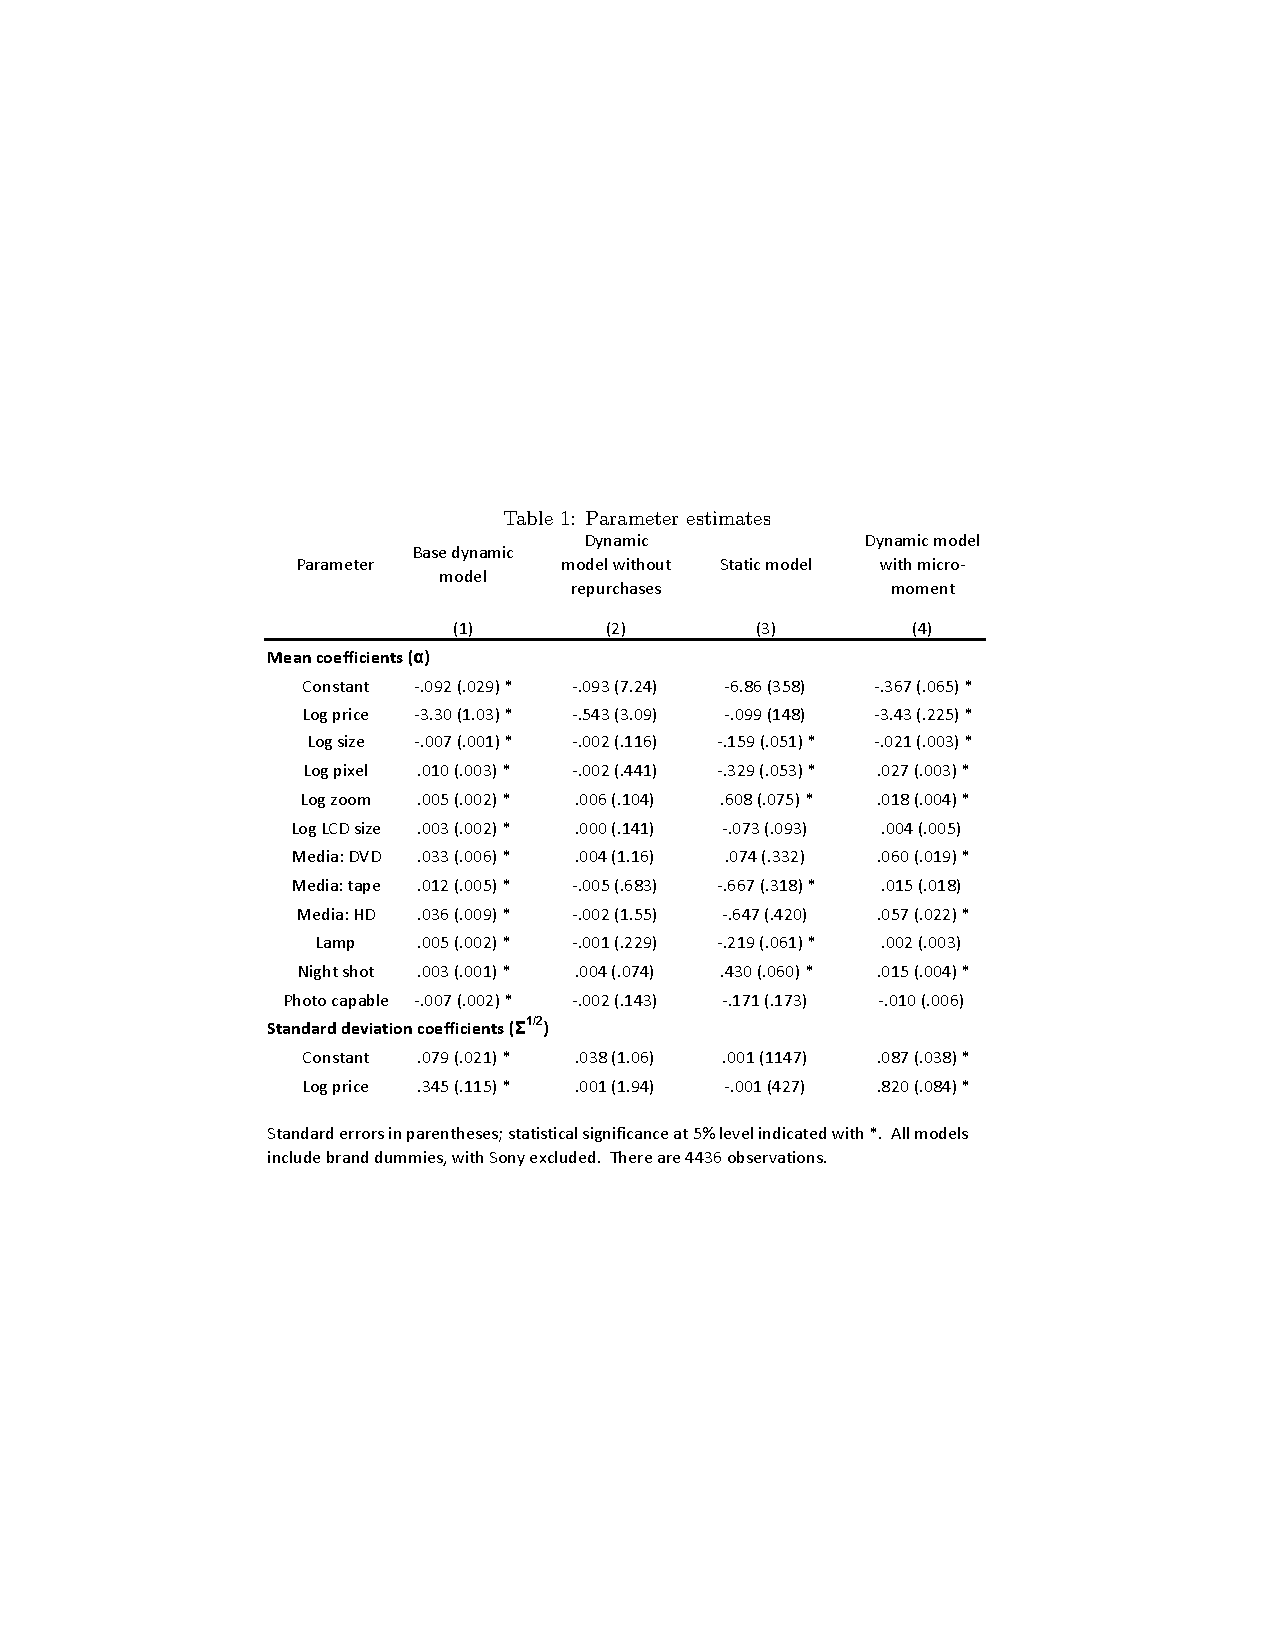
\includegraphics[width=3in]{resources/gandrtable1.pdf}
\end{center}
\end{figure}
\end{frame}

\begin{frame}{G\&R Robustness}
\begin{figure}[htbp]
\begin{center}
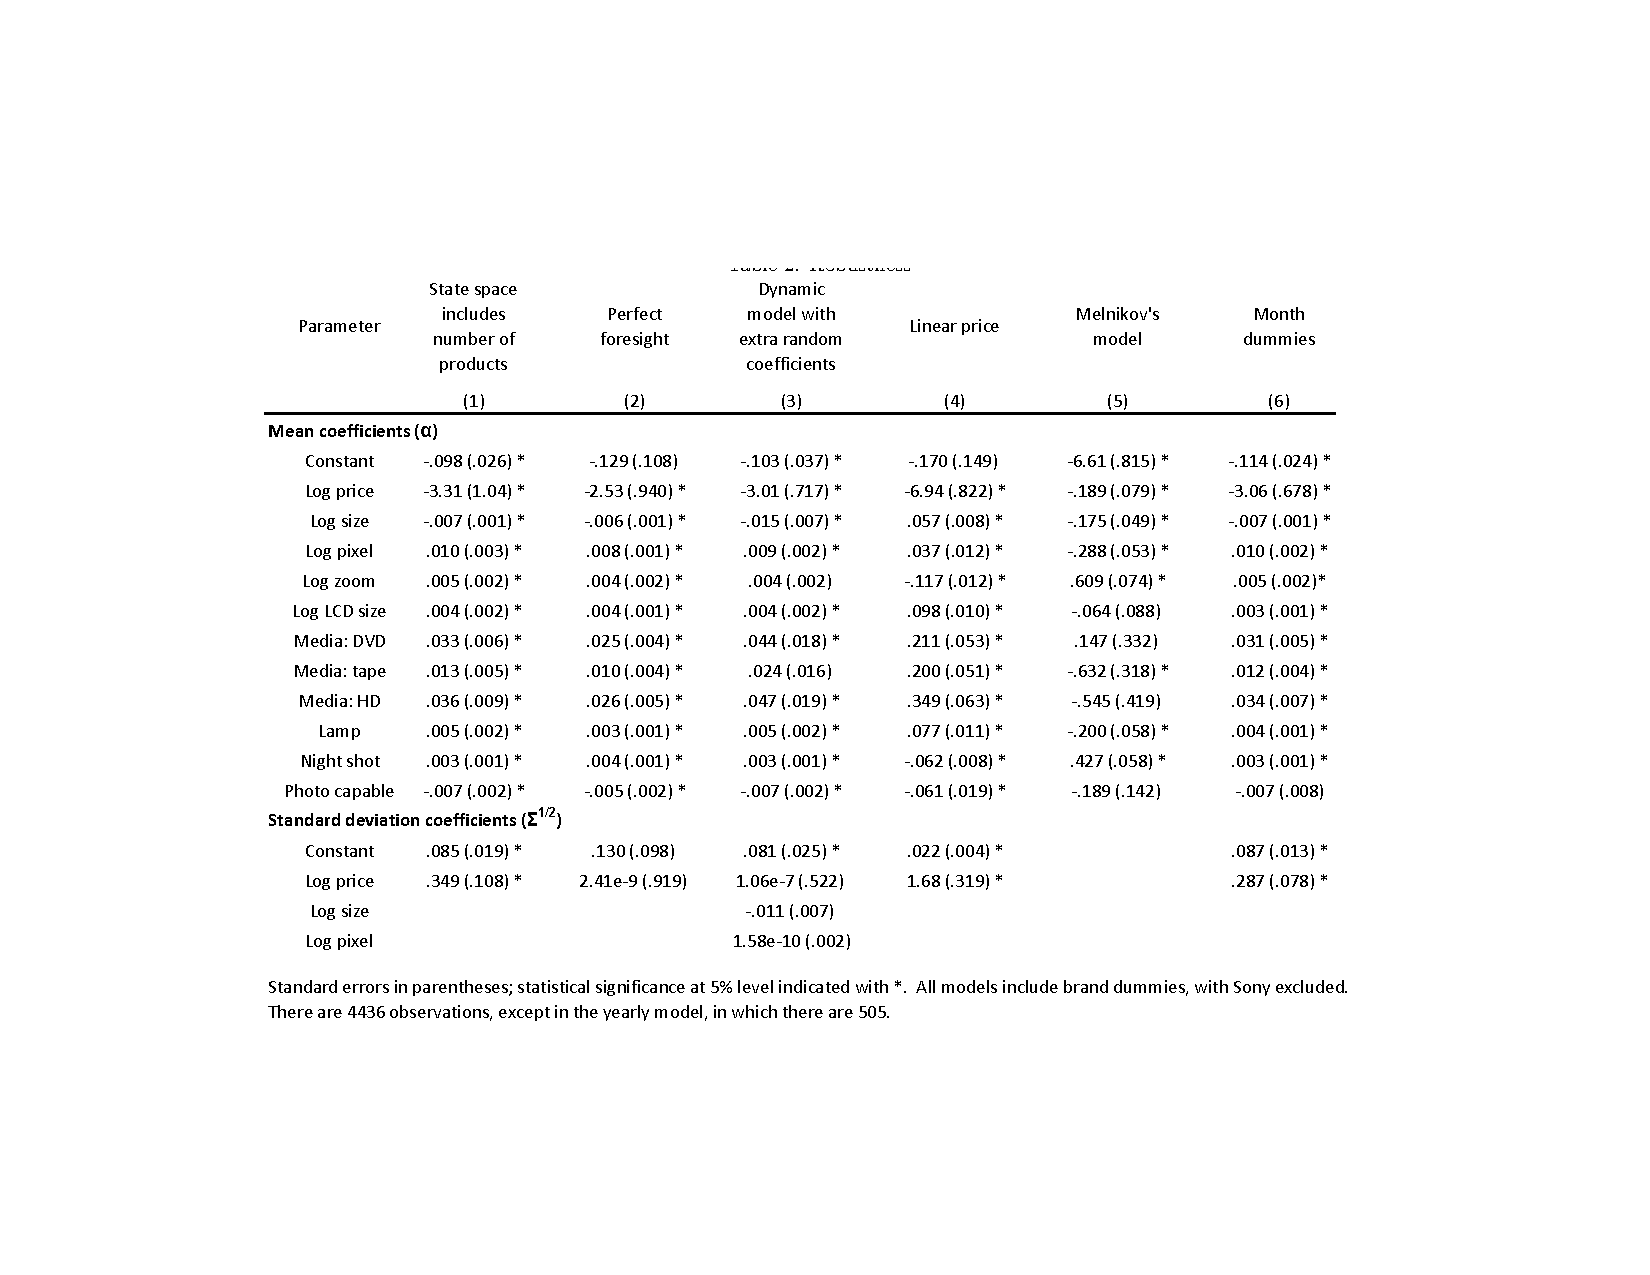
\includegraphics[width=4in]{resources/gandrtable2.pdf}
\end{center}
\end{figure}
\end{frame}


\begin{frame}{Results}
\begin{itemize}
\item Contrary to the static model, price coefficient is negative (as one would expect).
\item Coefficients on many product characteristics are intuitively appealing.
\item Allowing for repeated purchases generates more ``sensible'' results.
\item ``Better results'' from a dynamic model may be due to the fact that people wait to purchase because of the expectations of price declines and not directly because of high prices.
\item Unlike the static model, in dynamic setup the explanation of waiting does not conflict with consumers buying relatively high-priced products.
\item A variety of robustness measures show that the major simplifying assumptions about the dynamics in the model are broadly consistent with the data.
\end{itemize}
\end{frame}

\begin{frame}{Perfect Foresight}
G\&R Report similar elasticities in the perfect foresight case. We make the following simplification
\begin{eqnarray*}
E_{\Omega'}[ EV_i (f_{i0}, \delta_{i,t+1}) |\delta_{i,t}] )] = EV_i (f_{i0}, \delta_{i,t+1})
\end{eqnarray*}
This saves us a lot of headaches:
\begin{itemize}
\item No more integration/interpolation
\item We can solve the problem on the grid!
\item No more belief regressions
\end{itemize}
\end{frame}
%
%\begin{frame}{Conlon (2014)}
%Conlon (2014) suggests an alternate formulation of the problem.\\
%\vspace{0.25cm}
%Assume briefly that there are no upgrades $f_{i0t} = 0$, as well as perfect foresight:
%\begin{eqnarray*}
%E_{\Omega'}[ EV_i (f_{i0}, \delta_{i,t+1}) |\delta_{i,t}] )] &=& EV_i (f_{i0}, \delta_{i,t+1})  = v_{it} 
%\end{eqnarray*}
%\begin{eqnarray*}
% v_{it} \equiv EV_i(f_{i0}, \delta_i) &=& \log\left[ \exp( \beta v_{i,t+1})+ \exp(\delta_i)  \right] + \eta \\
%\end{eqnarray*}
%But we can always add back in the rational expectations error $v_{it} + \alert{\epsilon_{i,t}}$.
%\begin{eqnarray*}
%s_{ijt} = \int \frac{\exp[x_{jt}\beta + \xi_{jt} ]}{\exp[v_{i,t} + \epsilon_{i,t}] + \sum_k \exp[x_{jt}\beta + \xi_{jt} ]} f(\epsilon_{i,t})
%\end{eqnarray*}
%
%\end{frame}
%
%\begin{frame}{The Estimation Problem}
%We need to solve $\forall i, t $:
%\begin{eqnarray*}
%S_{jt}&=& \sum_i w_i s_{ijt}\\
%f_{ijt} &=& \overline{\alpha} x_{jt} + \xi_{jt} + \sum_l \sigma_l x_{jl} \nu_{il} \\
%s_{ijt} &=& \exp[f_{ijt} - \alpha_i p_{jt} - v_{it} ]\\
%v_{it} &=& \log\left[ \exp( \alert{\beta v_{i,t+1}} )+ \exp(\delta_{it})  \right] + \eta\\
%\delta_{it}&=& \log \left( \sum_j \exp[ f_{ijt}  -\alpha_i p_{jt} ]  \right)\\
%w_{i,t+1} &=& w_{i,t} \left(1-\sum_j s_{ijt} \right)\\
%\end{eqnarray*}
%Note: that this nests static demand $\alert{\beta} = 0$
%\end{frame}

\begin{frame}{Alternative Perspective on Beliefs}
Recall our objective:
\begin{itemize}
\item Plug in an unbiased estimate for the ``no-purchase'' utility.
\item Under perfect foresight this is just the inclusive value of tomorrow's market $\delta_{i,t+1}$  appropriately discounted: $\sum_{k=1}^{T-k} \beta^{t+k} \delta_{i,t+k}$.
\item Different ways to think about \alert{rational expectations}
\begin{itemize}
\item Expectational error of some or all of $\delta_{i,t+k}$'s.
\item Expectational error in today's reservation utility.
\end{itemize}
\end{itemize}
\end{frame}


\begin{frame}{Endogeneity and Instruments}
\footnotesize
\begin{itemize}
\item Dynamics mean we  \alert{lean harder on the assumption of exogenous product characteristics} 
\item In one period we can take characteristics as given, but in many periods this becomes less palatable (Do cameras exogenously improve over time?).
\item Endogeneity: price is endogenous while other product characteristics are not, i.e. $x_{jt}$. (Size,Resolution, etc.)
\item Price is chosen by the firms possibly after observing $\xi_{jt}$ and, hence, is endogenous.
\item Instruments: use variables that affect the price-cost margin, e.g. measures of how crowded a product is in characteristics space, which effects price-cost margin and the substitutability across products.
\begin{enumerate}
\item  all of the product characteristics in x;
\item mean product characteristics for a given firm;
\item mean product characteristics for all firms;
\item the count of products offered by the firm and by all firms.
\item changes in costs over time?
\end{enumerate}
\end{itemize}
\end{frame}


%
%\begin{frame}{The Estimation Problem}
%We need to solve $\forall i, t $:
%\begin{eqnarray*}
%S_{jt}(\theta) &=& \sum_i w_i s_{ijt}(f_{i0t},\delta_{it})\\
%f_{ijt} &=& \overline{\alpha}^x x_{jt} + \xi_{jt} + \sum_l \sigma_l x_{jl} \nu_{il} \\
%s_{ijt} &=& \frac{\exp[f_{ijt} - \alpha_i p_{jt} + \beta v_{i,t+1}] }{\exp [v_{it} ]}\\
%v_{i,t} &=& \log\left[ \alert{\exp(\beta v_{i,t+1})} + \exp(\delta_i)  \right]\\
%\delta_{it} &=& \log \left( \sum_j \exp[ f_{ijt}  -\alpha_i p_{jt} +\alert{\beta  v_{i,t+1}}]  \right)\\
%w_{i,t+1} &=&h(w_{i,t},s_{ijt})
%\end{eqnarray*}
%The only difference between this and BLP (in red).
%\end{frame}
%

%\begin{frame}{The Estimation Problem}
%We need to solve $\forall i, t $:
%\begin{eqnarray*}
%s_{ijt} &=& \exp[f_{ijt} - \alpha_i p_{jt} + \beta v_{i,t+1} - v_{i,t}] \\
%v_{i,t} &=& \log\left[ \alert{\exp(\beta v_{i,t+1})} + \exp(\delta_{it})  \right]\\
%\delta_{it} &=& \log \left( \sum_j \exp[ f_{ijt}  -\alpha_i p_{jt} +\alert{\beta  v_{i,t+1}}]  \right)\\
%\exp[v_{i,t} - \beta v_{i,t+1}] &=& \frac{ \exp(\beta v_{i,t+1})+ \exp(\delta_{it})} {\exp[\beta v_{i,t+1}]} \\
%&=& 1 + \exp{\delta_{it} - 
%\end{eqnarray*}
%\end{frame}

%\begin{frame}
%\frametitle{Adoption Problem}
%We'll begin by considering an adoption problem.
%\begin{itemize}
%\item Consumers make only one purchase decision
%\item Now we don't need to keep track of flow utilities in every period \alert{because you never purchase again}.
%\item Problem becomes an \textit{optimal stopping problem}
%\item Only keep track of value function for consumers with no durable.
%\item If consumers know future characteristics of products including $\epsilon_{ijt}$ then this is just a $J \times T$ static problem.
%\end{itemize}
%\vspace{0.5cm}
%We can assume that consumers receive PDV of entire future stream of utility payments $u_{i0t}$ when they make a purchase.
%\begin{eqnarray*}
%V_i(u_{i0t},\varepsilon_{i t}, \Omega_t) &=& 
%&& \max_j \underbrace{u_{ijt} + \beta E_{\Omega}[ E_{\varepsilon} V_i ( \varepsilon_{it}, \Omega_{t+1}) |\Omega_{t} ]  \}}_{\tilde{u}_{ijt}}
%\end{eqnarray*}
%\end{frame}

%
%\begin{frame}
%\frametitle{Solving the Adoption Problem}
%\begin{itemize}
%\item It is now impossible for $\overline{u}_{i0t}$ to change over time except through $\varepsilon_{i0t}$.
%\item And since $\tilde{u}_{ijt}$ is all paid at once we might as well normalize $\overline{u}_{i0t} = 0$.
%\item[¥]
%¥ Helpful to write: $EV_i(\Omega_t)= \int V_i(\varepsilon_{it},  \Omega_t)f(\varepsilon)$ \alert{Rust's Trick}
%\end{itemize}
%\begin{eqnarray*}
%V_i(u_{i0t},\varepsilon_{i t}, \Omega_t) &=& \max \{ u_{i0t} + \beta E[ E_{\varepsilon} V_i (u_{i0t}, \varepsilon_{it}, \Omega_{t+1}) |\Omega_{t} ] , \max_j \alert{\tilde{u}_{ijt}} \}
% \\
% &=& \max \{\beta E_{\Omega}[ EV_i(\Omega_{t+1}) |\Omega_{t} ] +\varepsilon_{i0t}, \max_j \tilde{u}_{ijt} \}
% \end{eqnarray*}
% \vspace{-0.5cm}
%\end{frame}
%
%
%
%\begin{frame}
%\frametitle{Logit Inclusive Value Trick}
%The $E_{\varepsilon}[ \max_j \tilde{u}_{ijt}]$ has a closed form expression based on the logit inclusive value:
%\begin{eqnarray*}
%\delta_{it} = E_{\varepsilon}[\max_j \tilde{u}_{ijt} ] &=& \log \sum_j \exp(x_{jt} \alpha_i^x - \alpha_{i}^p p_{jt} +  \xi_{jt})\\
%EV_i(\Omega_t)&=& \max \{\beta E_{\Omega}[ EV_i(\Omega_{t+1}) |\Omega_{t} ] +\varepsilon_{i0t}, \max_j \tilde{u}_{ijt} \}\\
%&=& \max \{\beta E_{\Omega}[ EV_i(\Omega_{t+1}) |\Omega_{t} ] +\varepsilon_{i0t}, \delta_{it} \}\\
%&=& \log \left( \exp[\beta E_{\Omega}[ EV_i(\Omega_{t+1}) |\Omega_{t} ] +  \exp[\delta_{it}] \right) + \eta
% \end{eqnarray*}
%Where $\eta = 0.577215665$ (Euler's Constant).
%\end{frame}
%
%\begin{frame}
%\frametitle{Inclusive Value Sufficiency}
%\begin{eqnarray*}
%EV_i(\Omega_t) &=& \log \left( \exp[\beta E_{\Omega}[ EV_i(\Omega_{t+1}) |\Omega_{t} ] +  \exp[\delta_{it}] \right) + \eta
% \end{eqnarray*}
%The fact that the expected value function depends recursively on itself and $\delta_{it}$ (Inclusive Value) leads to the following assumption.
%\begin{block}{Inclusive Value Sufficiency}
%If $\delta(\Omega) = \delta(\tilde{\Omega})$ then $g(\delta(\Omega') | \Omega)= g(\delta(\tilde{\Omega'}) | \tilde{\Omega})$
%\end{block}
%\end{frame}
%

\end{document}













































